\subsection{METODOLOG\'IAS DE VALUACI\'ON DE NEGOCIOS E INTANGIBLES}. 

Se aplicaron \textcolor{secundario}{dos t\'ecnicas de valuaci\'on de negocios} y a su vez \textcolor{principal}{dos t\'ecnicas de valuaci\'on de activos intangibles}, con amplia aceptaci\'on en el medio financiero (\autoref{fig:metodologias} y \autoref{fig:metodologias_2}), con el objeto de determinar el \textcolor{secundario}{valor razonable de la marca}.\\

\begin{figure}[H]
\centering
\caption{Metodolog\'ias de Valuaci\'on de negocios\label{fig:metodologias}}\vspace{10pt}
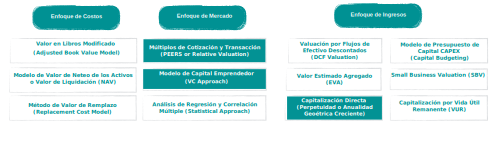
\includegraphics[width=.8\textwidth]{\rutaImagenes/metodologias_valuacion_negocio}\\

\caption{Metodolog\'ias de Valuaci\'on de Activos Intangibles\label{fig:metodologias_2}}
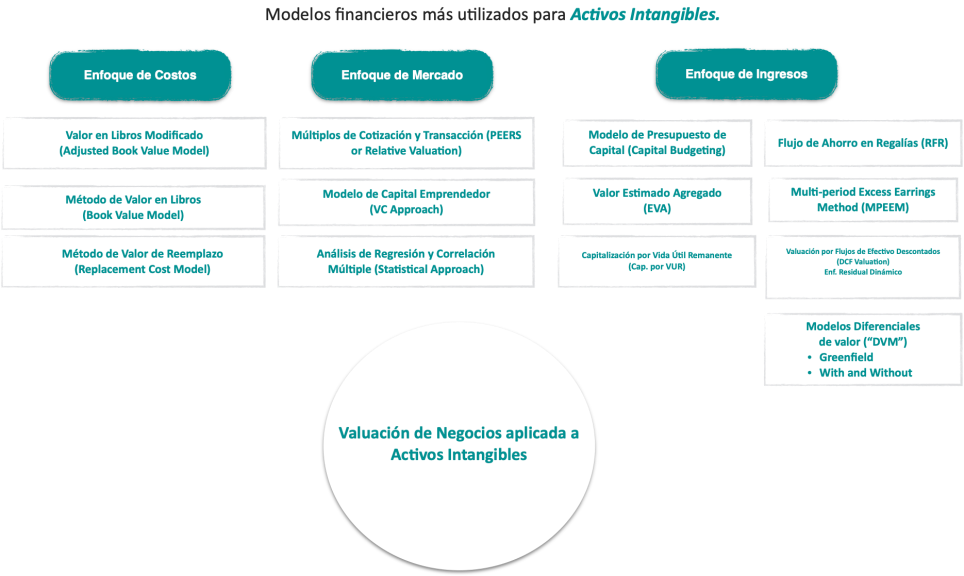
\includegraphics[width=.4\textwidth]{\rutaImagenes/metodologias_valuacion_intangibles}\\

\end{figure}

Los activos intangibles consisten en una verdadera inversi\'on para el negocio. Por lo anterior, el perito valuador parti\'o de las hip\'otesis planteadas en el siguiente diagrama de reconocimiento (\autoref{fig:metodologias_3}):

\begin{figure}[H]
\centering
\caption{Diagrama de reconocimiento de la NIF C-8\label{fig:metodologias_3}}
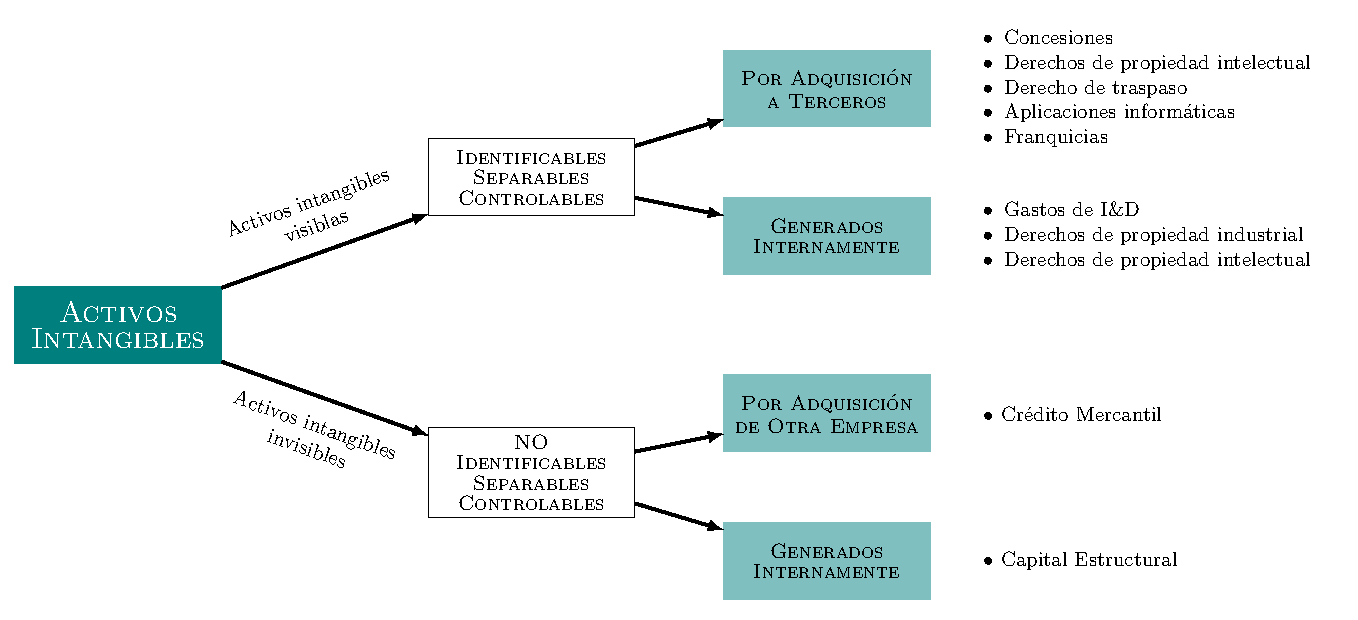
\includegraphics[width=10cm]{\rutaImagenes/NIF_C8}\\
\end{figure}

